Este capítulo apresenta os resultados obtidos através da realização do presente trabalho. Assim, ele descreve os testes de comparação realizados entre os modelos de tradução apresentados submetidos aos textos de domínio geral e específico utilizando métricas como eficiência computacional e métricas de qualidade de tradução.



Os gráficos de métricas de qualidade também permitem observar a distribuição dos resultados obtidos para cada modelo, e não apenas os valores médios. Para essa leitura, as caixas representam o intervalo entre o primeiro e o terceiro quartis, concentrando a metade central das observações. O losango preto representa a mediana, enquanto a linha laranja representa a média. Os prolongamentos da caixa indicam os limites inferior e superior do intervalo principal, relacionados aos valores mínimo e máximo nele contidos. Pontos isolados além desses limites representam observações fora desse intervalo e indicam sentenças com comportamento diferente do conjunto predominante.

Essa representação permite comparar a posição central e a dispersão dos resultados entre os modelos. Caixas ou intervalos mais altos indicam maior variação entre as sentenças avaliadas, enquanto caixas mais baixas indicam resultados mais concentrados. Da mesma forma, a distância entre a média e a mediana auxilia na identificação de distribuições assimétricas. Portanto, mesmo sem considerar análises estatísticas adicionais, os gráficos evidenciam diferenças no comportamento dos modelos quanto ao desempenho típico, à variação dos resultados e à ocorrência de valores extremos.

\section{Métricas de qualidade}
Esta seção apresenta os resultados obtidos pelos modelos avaliados a partir das métricas BLEU, BERTScore e chrF. A análise considera separadamente os textos gerais e os textos específicos, permitindo verificar tanto o desempenho relativo entre os modelos quanto a influência do tipo de texto sobre os resultados.

Como todos os modelos foram submetidos às mesmas sentenças de entrada e avaliados em relação às mesmas traduções de referência, as diferenças observadas nas métricas permitem realizar uma comparação direta entre os modelos nas condições estabelecidas no experimento. Essa padronização foi definida na metodologia justamente para garantir condições equivalentes entre os modelos.

\subsection{BLEU}

As figuras \ref{fig:bleu-general} e \ref{fig:bleu-specific} demonstram os resultados obtidos da métrica de qualidade \textit{BLEU} quando aplicados ao resultado das traduções geradas pelos modelos apresentados

\begin{figure}[H]
    \centering
    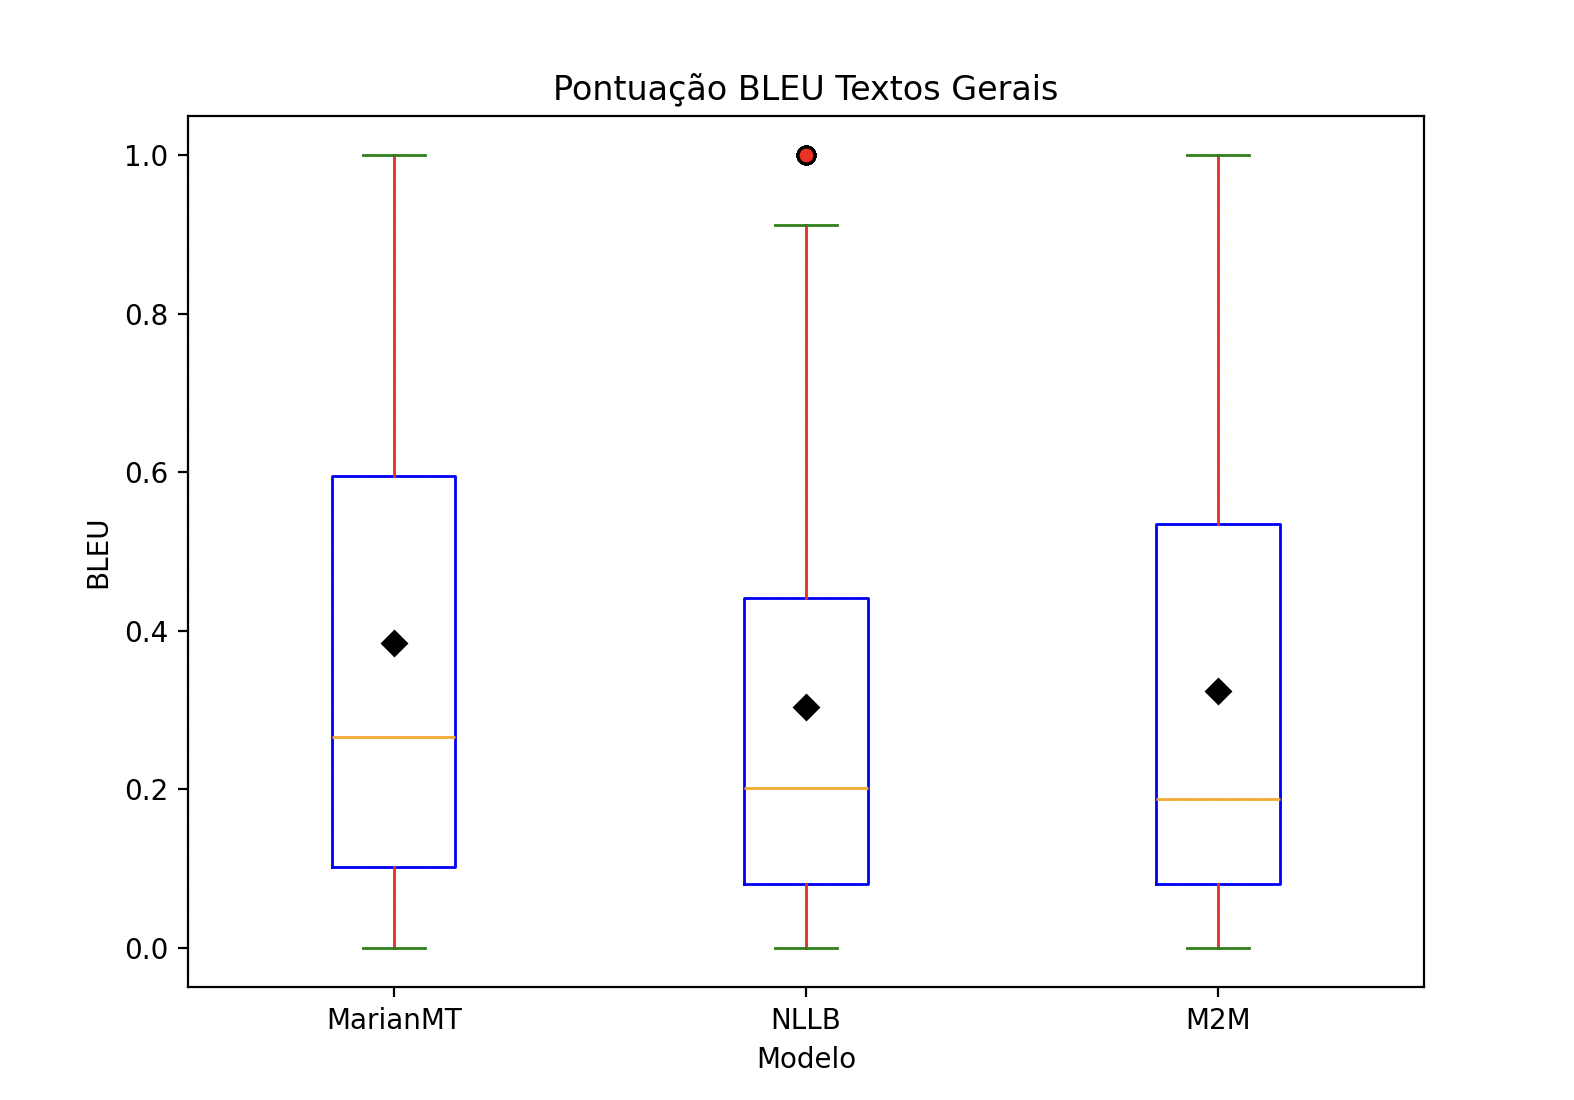
\includegraphics[width=0.7\textwidth]{Imagens/BLEU-GENERAL.png}
    \caption{\label{fig:bleu-general} Métrica BLEU por modelo e textos gerais}
    \legend{Fonte: autor}
\end{figure}

\begin{figure}[H]
    \centering
    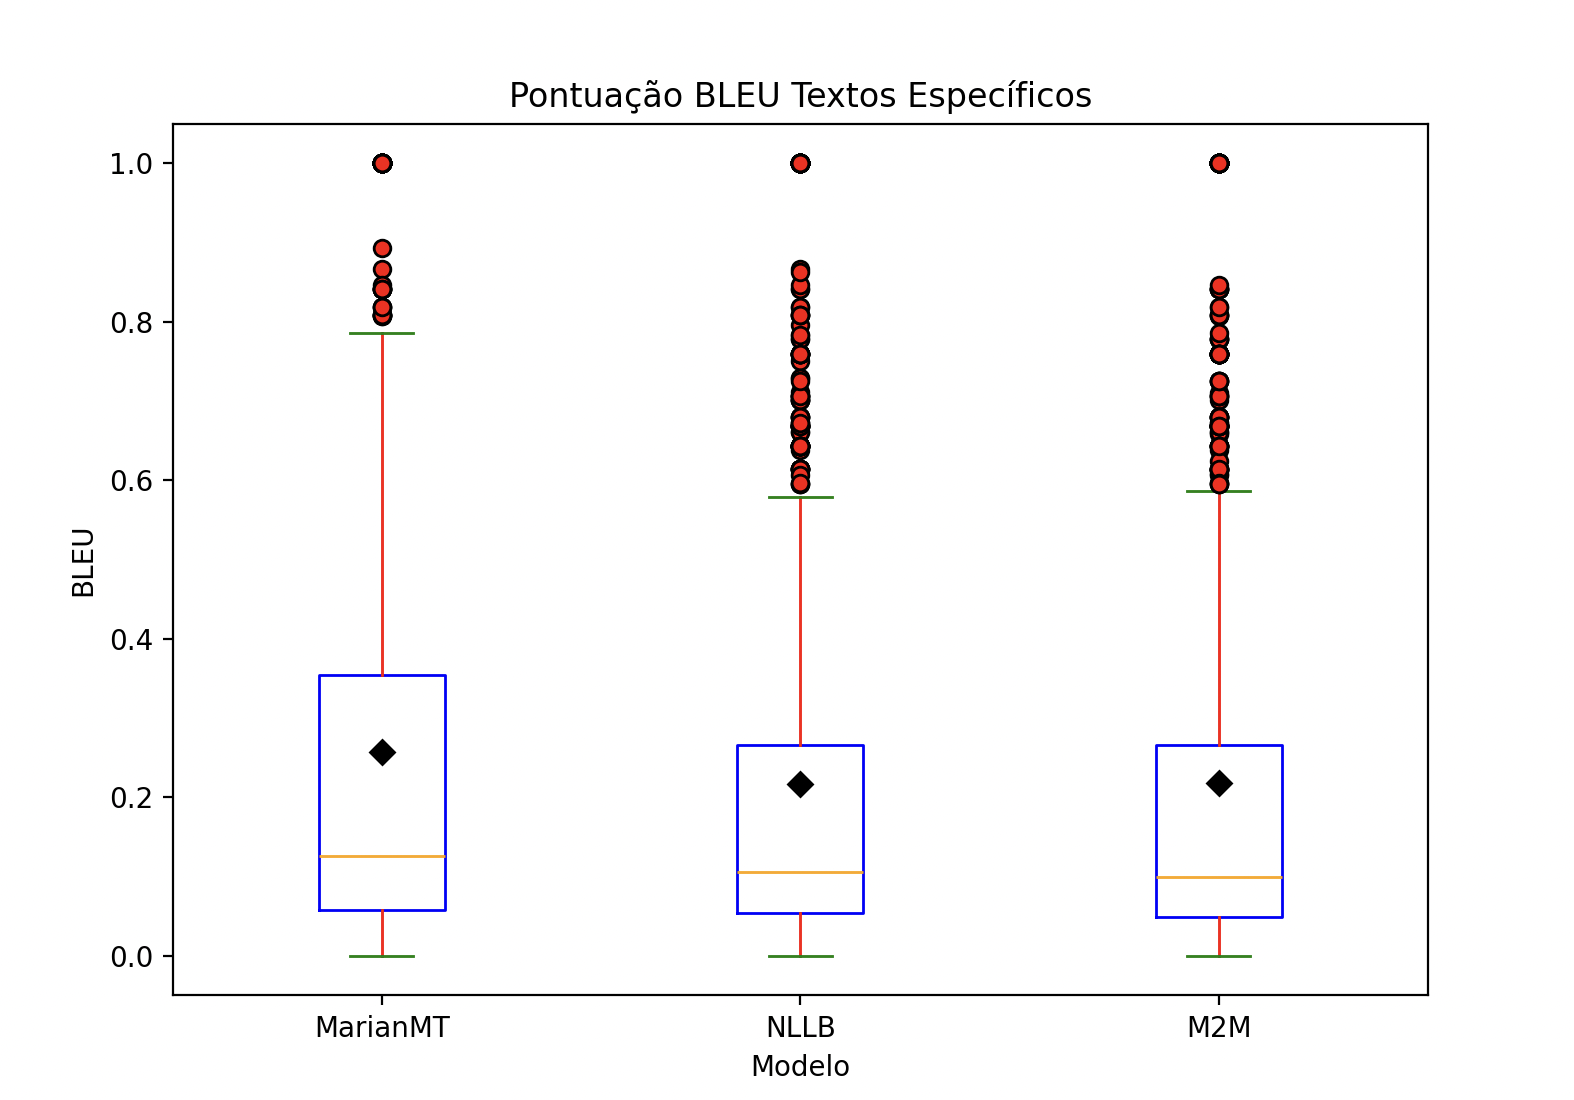
\includegraphics[width=0.7\textwidth]{Imagens/BLEU-SPECIFIC.png}
    \caption{\label{fig:bleu-specific} Métrica BLEU por modelo e textos específicos}
    \legend{Fonte: autor}
\end{figure}

Nos textos gerais, observa-se que o modelo Helsinki-NLP/opus-mt-tc-big-en-pt(MarianMT) apresentou o maior valor de BLEU entre os modelos avaliados. O facebook/m2m100-418M(M2M) apresentou resultado intermediário, enquanto o facebook/nllb-200-distilled-600M(NLLB) apresentou o menor valor entre os três modelos.

Nos textos específicos, observa-se novamente o melhor resultado para o MarianMT. Entretanto, a diferença entre os dois modelos restantes é menor: o M2M100 apresenta valor de BLEU de 0,218, enquanto o NLLB apresenta 0,217. O MarianMT, por sua vez, apresenta média de 0,258.

Ao comparar os dois tipos de texto, verifica-se uma redução nos valores de BLEU para os três modelos quando são considerados os textos específicos. O MarianMT apresentou redução de aproximadamente 32,8\%, passando de 0,384 nos textos gerais para 0,258 nos textos específicos.

Esse comportamento indica que, nas condições avaliadas, os textos específicos apresentaram maior dificuldade para os modelos em relação aos textos gerais segundo a métrica BLEU. A redução foi observada para todos os modelos, embora em diferentes magnitudes.

\subsection{BERTScore}

As Figuras \ref{fig:bertscore-general} e \ref{fig:bertscore-specific} apresentam os resultados obtidos pela métrica BERTScore para os textos gerais e específicos, respectivamente.

\begin{figure}[H]
    \centering
    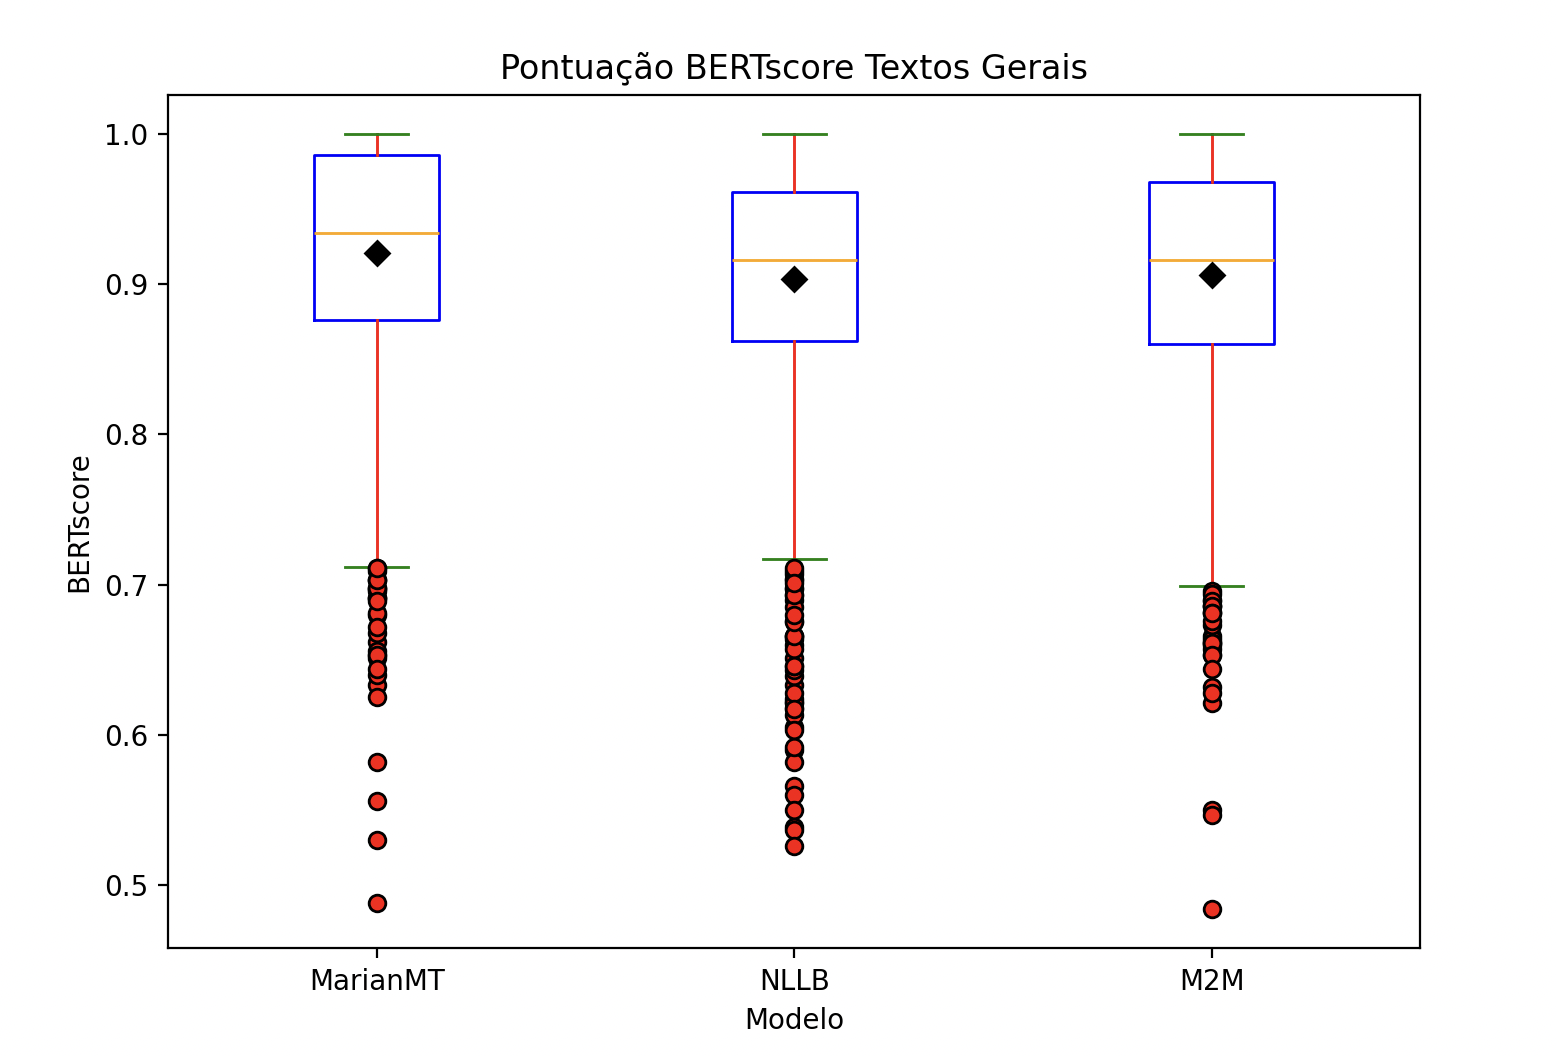
\includegraphics[width=0.8\textwidth]{Imagens/BERTSCORE-GERAL.png}
    \caption{\label{fig:bertscore-general} Métrica BERTScore por modelo e textos gerais}
    \legend{Fonte: autor}
\end{figure}

\begin{figure}[H]
    \centering
    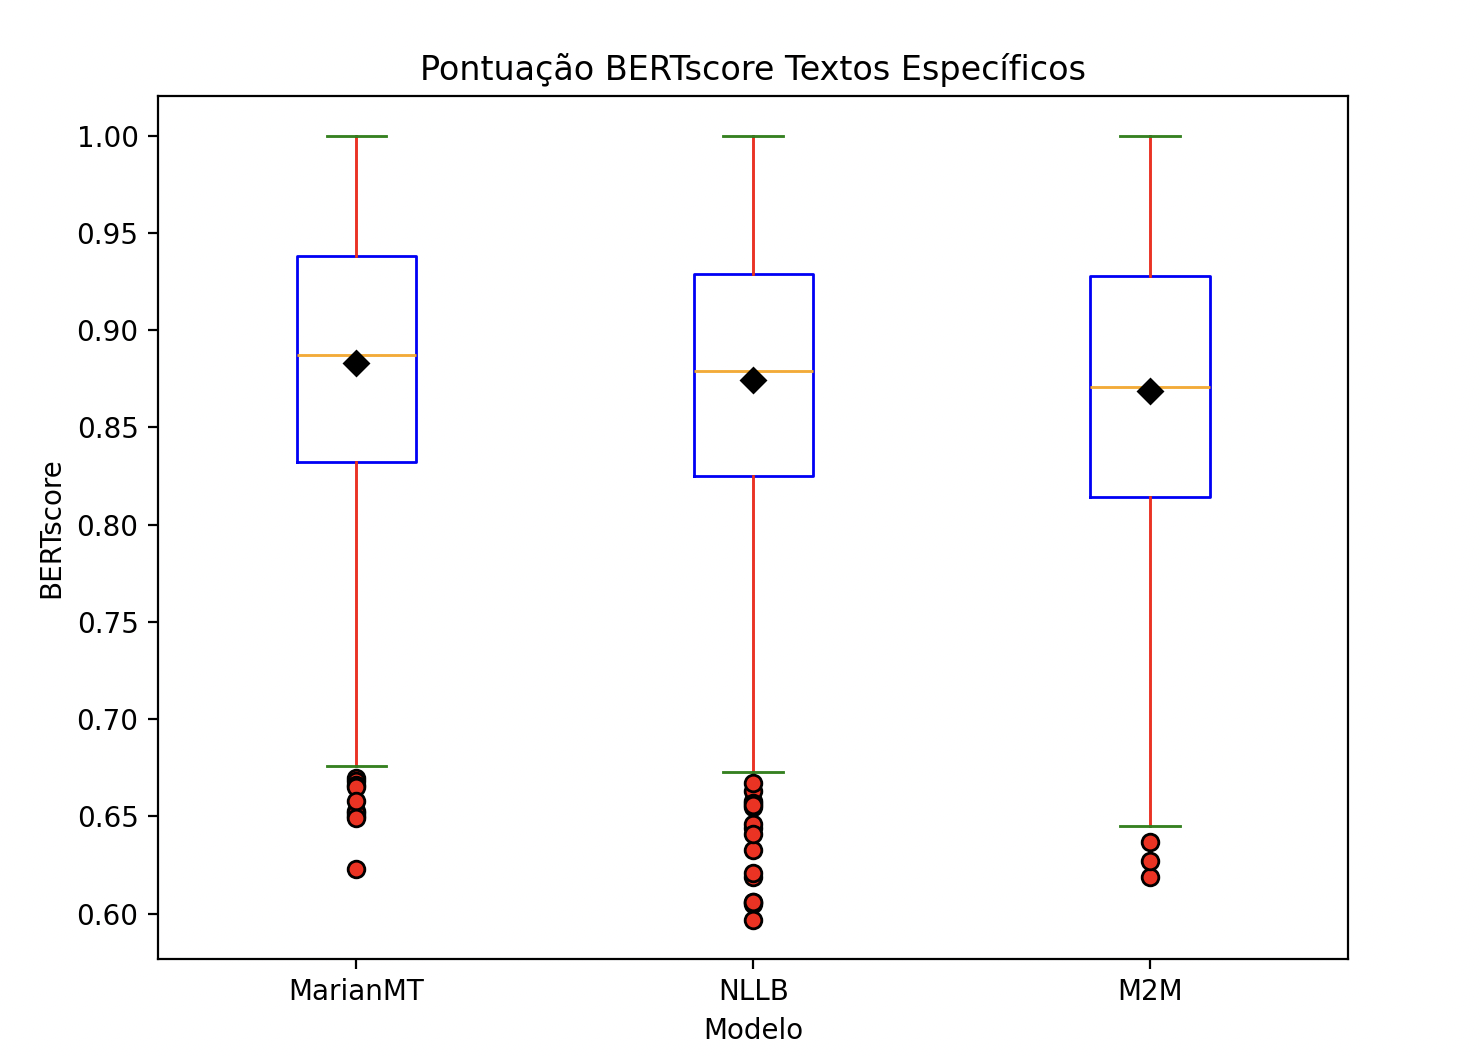
\includegraphics[width=0.8\textwidth]{Imagens/BERTSCORE-ESPECIFICO.png}
    \caption{\label{fig:bertscore-specific} Métrica BERTScore por modelo e textos específicos}
    \legend{Fonte: autor}
\end{figure}

Para os textos gerais, o MarianMT apresentou novamente o maior resultado, com média de 0,921. O M2M100 apresentou valor de 0,906, enquanto o NLLB apresentou 0,903. Dessa forma, embora a diferença entre NLLB e M2M100 seja pequena, o MarianMT apresentou vantagem sobre os demais modelos.Nos textos específicos, o comportamento geral foi mantido. O MarianMT apresentou o maior valor, com 0,883, seguido pelo NLLB, com 0,875, e pelo M2M100, com 0,869.

Assim como observado no BLEU, houve redução dos valores de BERTScore quando considerados os textos específicos. Entretanto, essa redução foi menos acentuada para o MarianMT, que passou de 0,921 para 0,883, correspondendo a uma redução aproximada de 4,1\%.

A diferença observada entre os dois tipos de texto indica que o domínio específico influenciou os resultados também segundo o BERTScore. Contudo, a menor redução observada nessa métrica, quando comparada ao BLEU, demonstra que o comportamento dos indicadores não é necessariamente equivalente em magnitude.


\subsection{chrf}

As Figuras \ref{fig:chrf-general} e \ref{chrf-specific} apresentam os resultados obtidos pela métrica chrF para os textos gerais e específicos.

\begin{figure}[H]
    \centering
    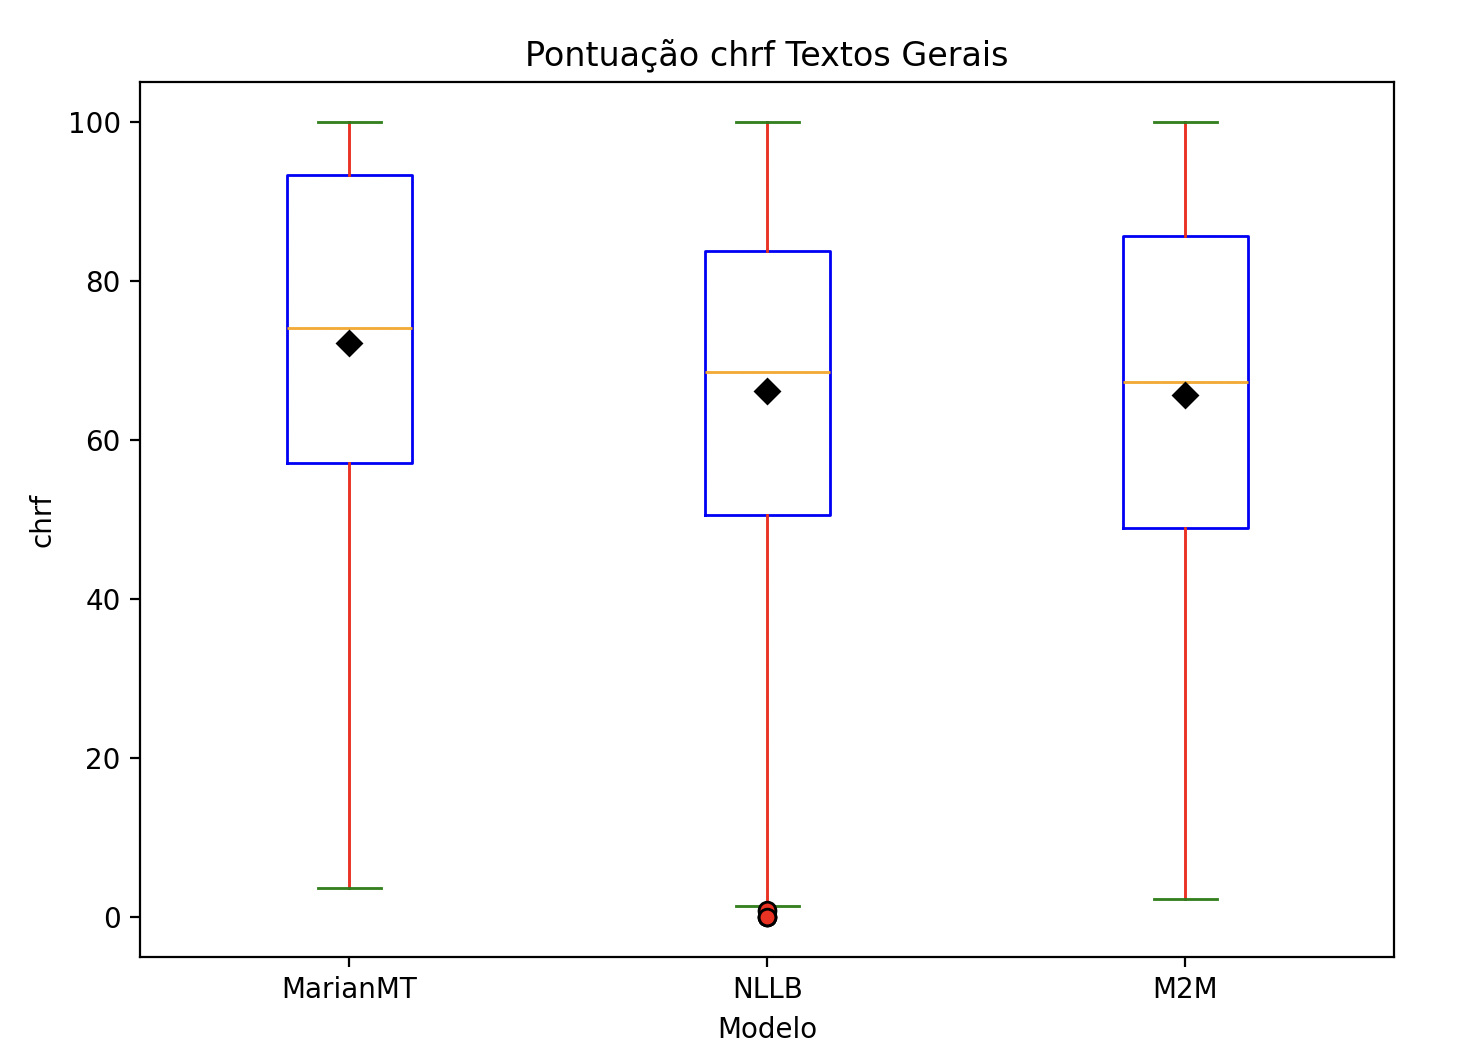
\includegraphics[width=0.8\textwidth]{Imagens/CHRF-GERAL.png}
    \caption{\label{fig:chrf-general} Métrica chrf por modelo e textos gerais}
    \legend{Fonte: autor}
\end{figure}

\begin{figure}[H]
    \centering
    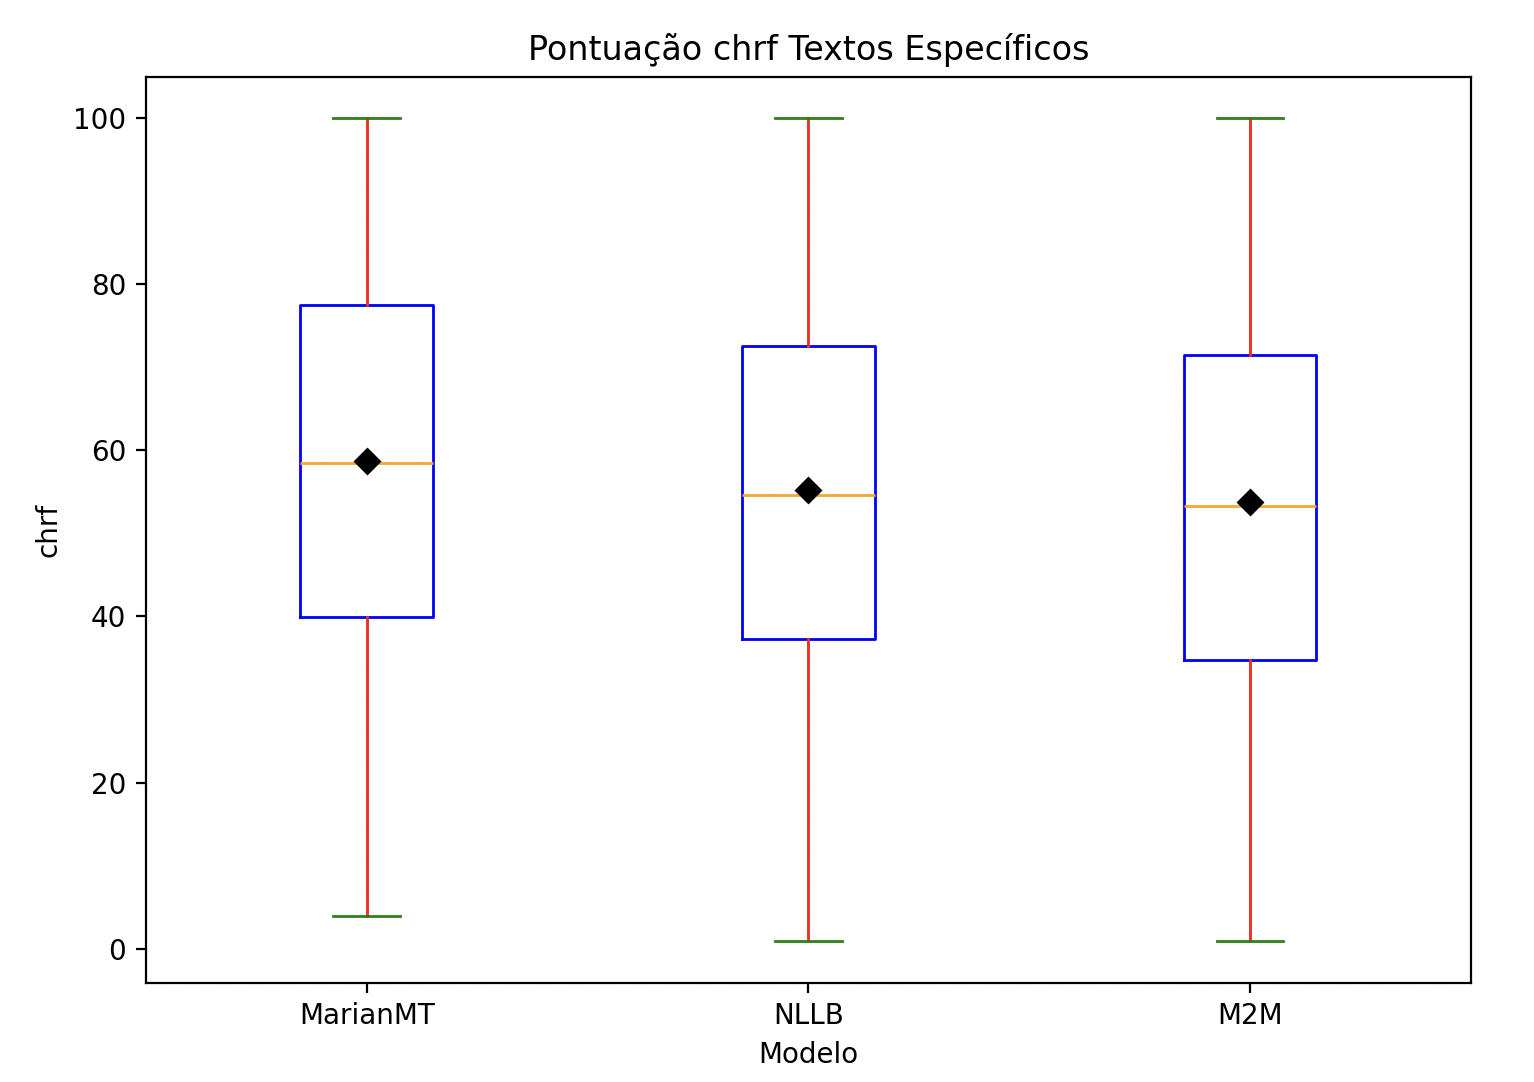
\includegraphics[width=0.8\textwidth]{Imagens/CHRF-ESPECIFICO.png}
    \caption{\label{chrf-specific} Métrica chrf por modelo e textos específicos}
    \legend{Fonte: autor}
\end{figure}

Nos textos gerais, o MarianMT apresentou o maior valor, com média de 72,185. O NLLB apresentou 66,196, enquanto o M2M100 apresentou 65,683. Dessa forma, o MarianMT apresentou vantagem sobre os demais modelos, enquanto a diferença entre NLLB e M2M100 foi relativamente pequena.Para os textos específicos, o MarianMT também apresentou o maior resultado, com 58,676. O NLLB apresentou 55,235, enquanto o M2M100 apresentou 53,842.

Assim como nas demais métricas, observa-se redução dos resultados para os textos específicos. No caso do MarianMT, o valor médio passou de 72,185 para 58,676, representando uma redução aproximada de 18,7\%.

Os resultados obtidos pelo chrF, portanto, acompanham a tendência observada nas demais métricas: o MarianMT apresenta o maior desempenho nos dois tipos de texto, enquanto os valores obtidos para os textos específicos são inferiores aos observados nos textos gerais.

Um aspecto a ser comentado, considerando a natureza dos gráficos apresentados, é a relação entre a média e a mediana, representadas, respectivamente, pela linha laranja e pelo losango preto. Observa-se que, nas métricas BERTScore e chrF, a média tende a se aproximar da mediana, indicando uma proximidade entre o valor médio e o valor central da distribuição dos resultados. Entretanto, para a métrica BLEU, esse padrão não se repete, uma vez que a média tende a apresentar valores superiores aos da mediana.

Em síntese, é possível observar uma tendência semelhante na distribuição dos valores das métricas BERTScore e chrF. Por outro lado, a métrica BLEU apresenta um comportamento distinto, caracterizado por médias superiores às medianas, o que pode indicar uma diferença na distribuição dos resultados.

\section{Eficiência Computacional}

A eficiência computacional dos modelos foi avaliada considerando o uso médio de CPU, o pico de memória RAM e o tempo de inferência. Os resultados completos são apresentados na Tabela \ref{table-efficiency} e nas Figuras \ref{fig:average-cpu}, \ref{fig:peak-memory} e \ref{fig:inference-time}.

\begin{table}[htbp]
  \centering
  \caption{Comparação de Desempenho e Recursos por Modelo e Tipo de texto}
  \vspace{0.5em}
  \label{table-efficiency}
  \setlength{\tabcolsep}{3pt}
  \begin{tabularx}{\textwidth}{>{\raggedright\arraybackslash}X l r r r r r}
    \toprule
    \textbf{Modelo} & \textbf{Base} & \textbf{CPU Média} & \textbf{CPU Máx.} & \textbf{Mem. Adic.} & \textbf{Pico Mem.} & \textbf{Tempo Inf.} \\
    \midrule
    Helsinki-NLP/\penalty0opus-mt-tc-big-en-pt & Geral & 53,8\% & 100,0\% & 247,30 MB & 6,24 GB & 2,592s \\
    Helsinki-NLP/\penalty0opus-mt-tc-big-en-pt & Específica & 55,7\% & 100,0\% & 247,55 MB & 6,26 GB & 2,222s \\
    \addlinespace
    facebook/\penalty0nllb-200-distilled-600M & Geral & 61,4\% & 100,0\% & 247,29 MB & 6,25 GB & 3,095s \\
    facebook/\penalty0nllb-200-distilled-600M & Específica & 62,2\% & 100,0\% & 247,50 MB & 6,27 GB & 2,563s \\
    \addlinespace
    facebook/\penalty0m2m100\_418M & Geral & 71,5\% & 100,0\% & 247,33 MB & 6,25 GB & 4,217s \\
    facebook/\penalty0m2m100\_418M & Específica & 73,6\% & 100,0\% & 247,55 MB & 6,27 GB & 3,621s \\
    \bottomrule
  \end{tabularx}
\end{table}

\begin{figure}[H]
    \centering
    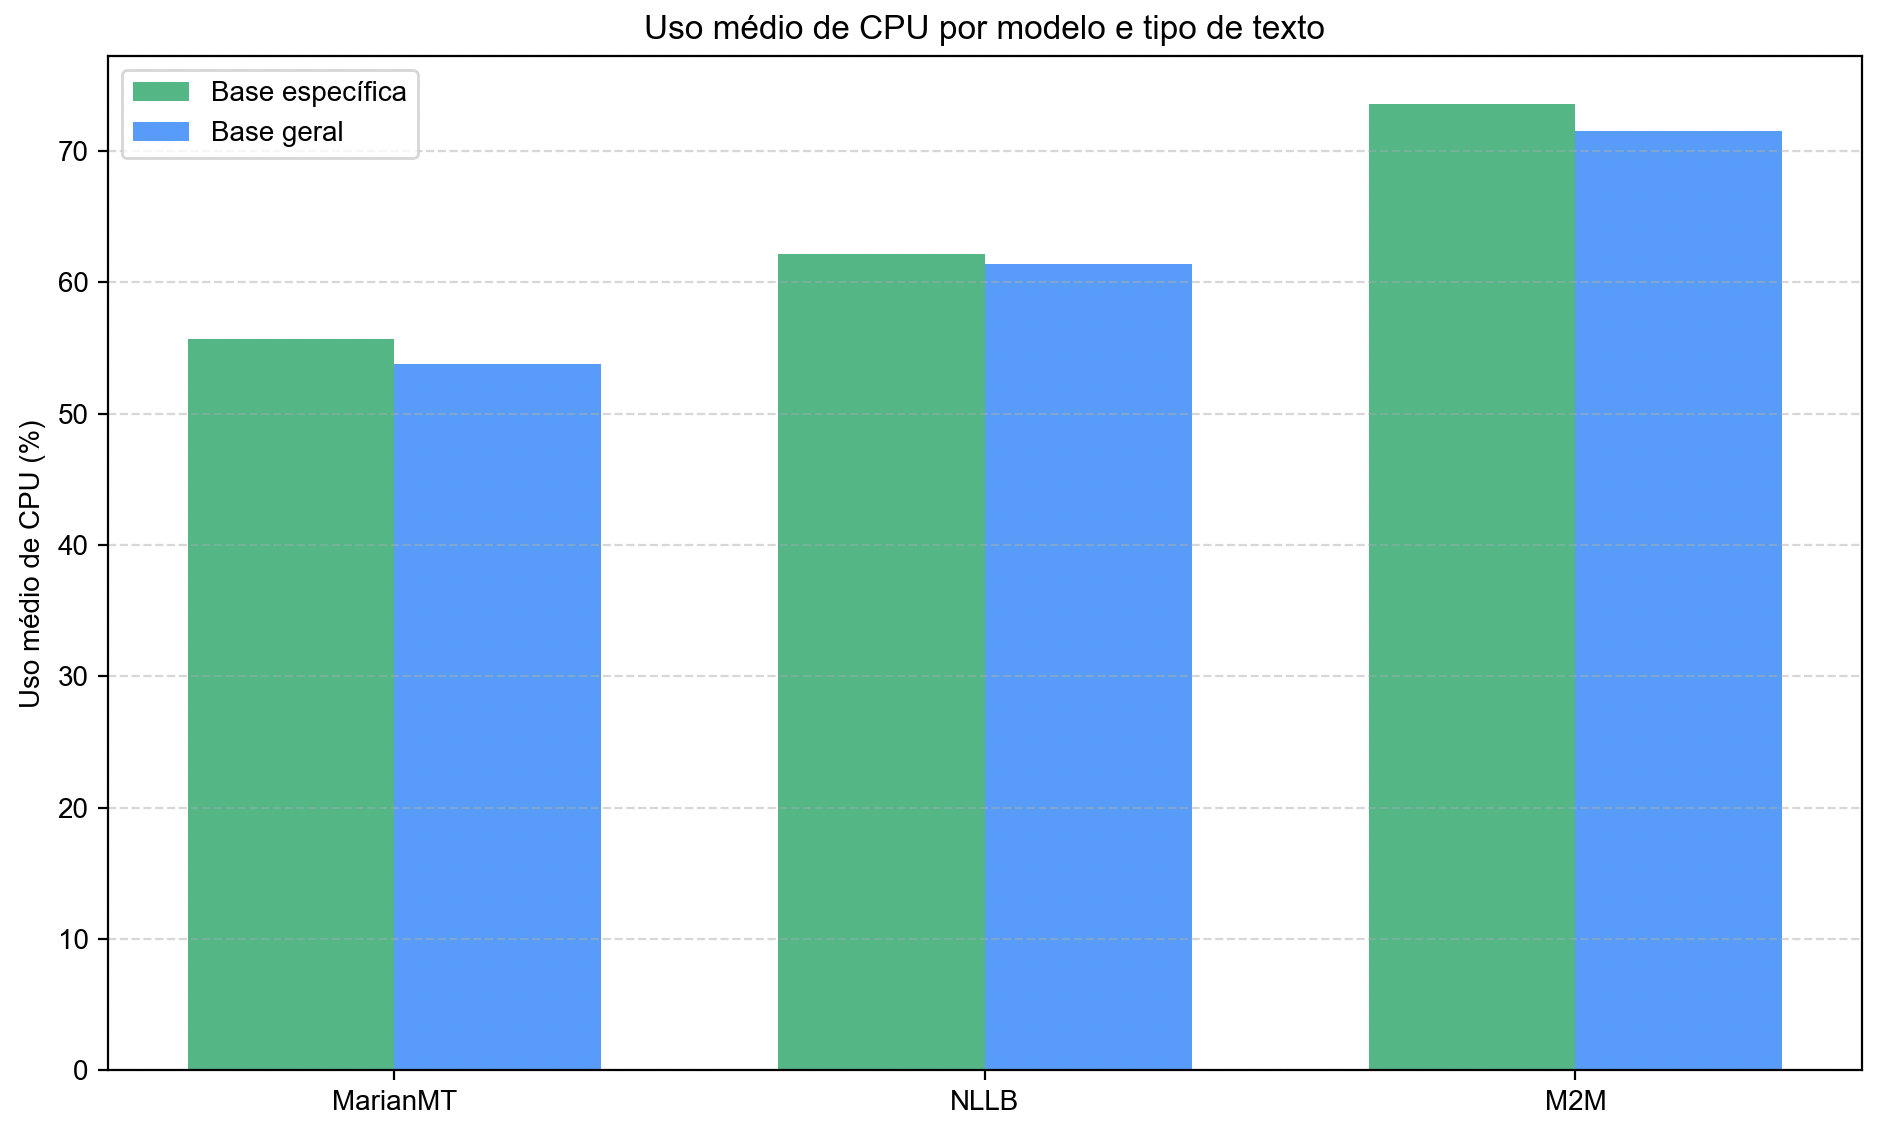
\includegraphics[width=0.9\textwidth]{Imagens/AVERAGE-CPU-USAGE.png}
    \caption{\label{fig:average-cpu} Uso médio de CPU por modelo e tipo de texto}
    \legend{Fonte: autor}
\end{figure}

\begin{figure}[H]
    \centering
    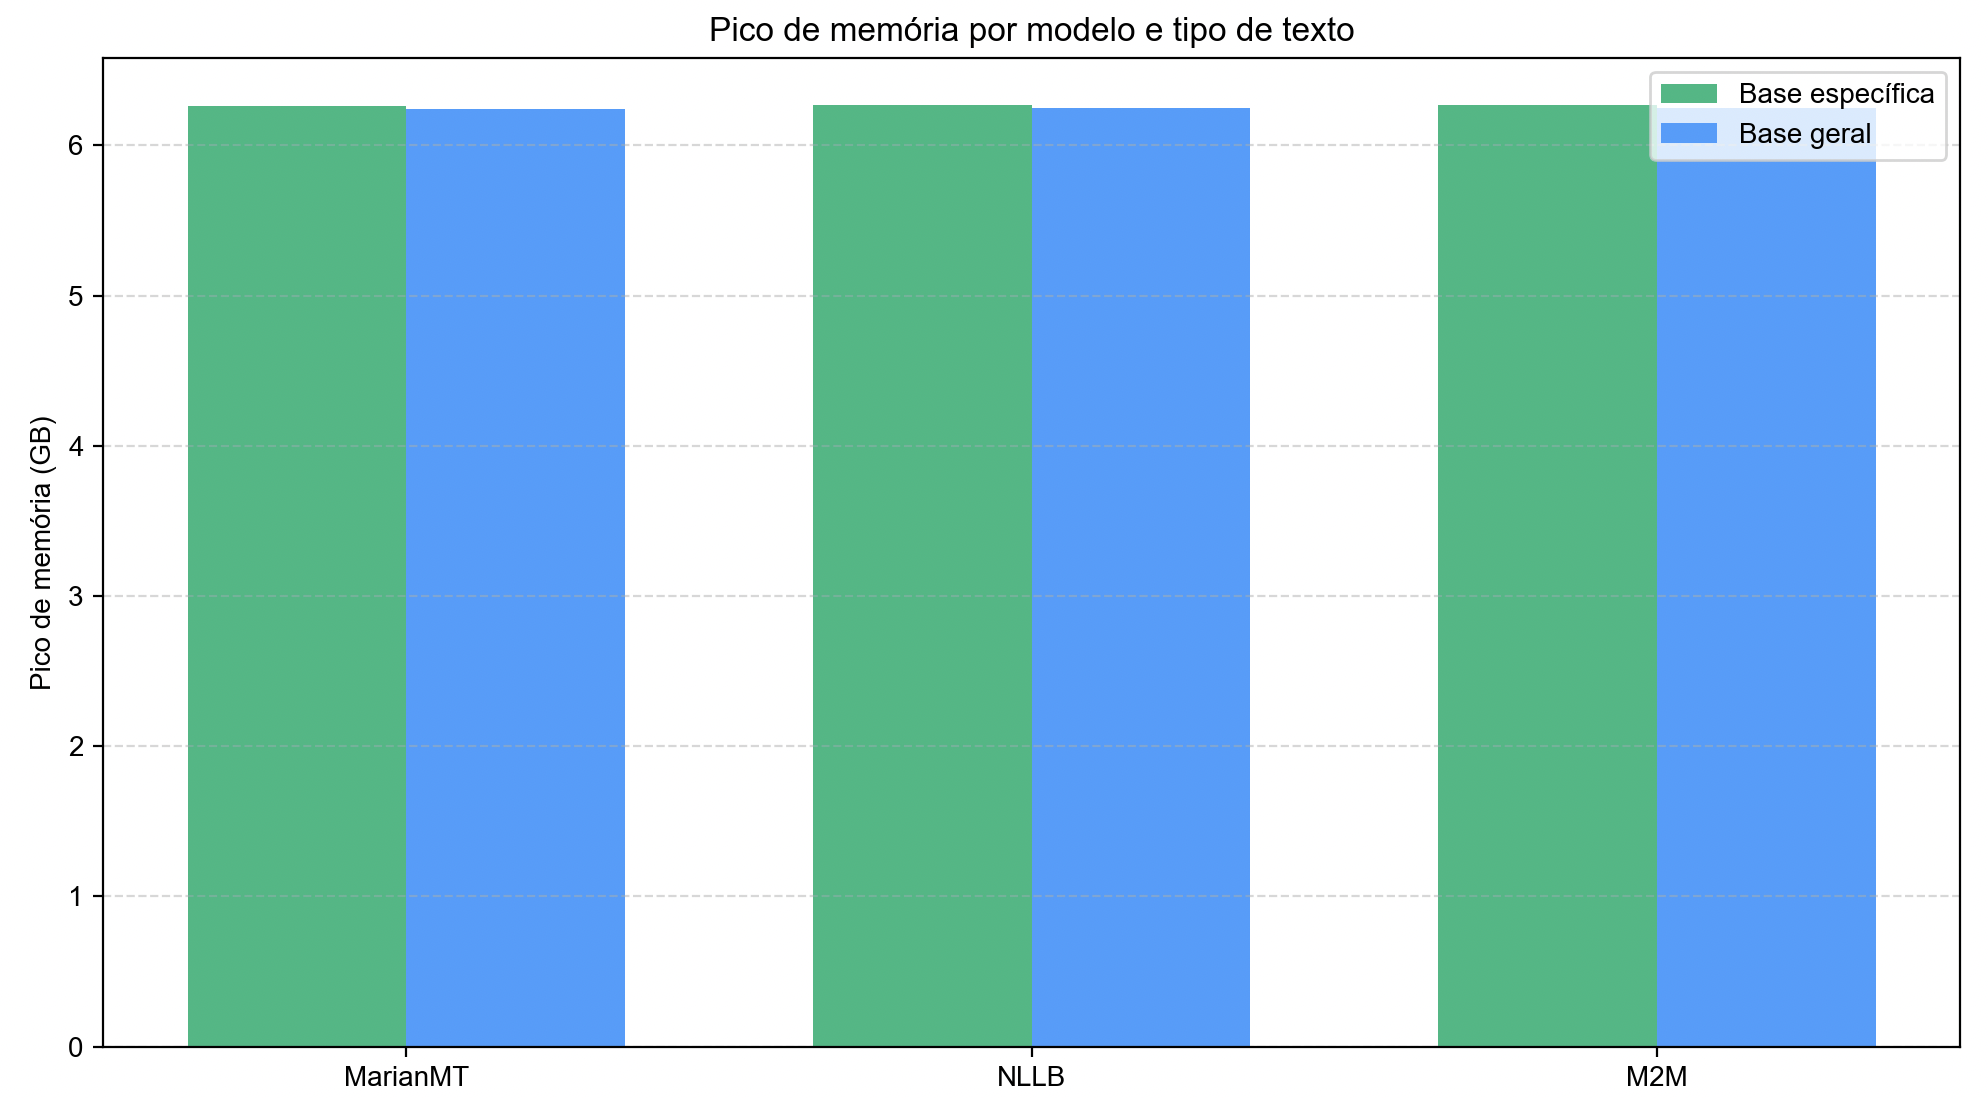
\includegraphics[width=0.9\textwidth]{Imagens/PEAK-MEMORY2.png}
    \caption{\label{fig:peak-memory} Pico de memória RAM utilizada por modelo e tipo de texto}
    \legend{Fonte: autor}
\end{figure}

\begin{figure}[H]
    \centering
    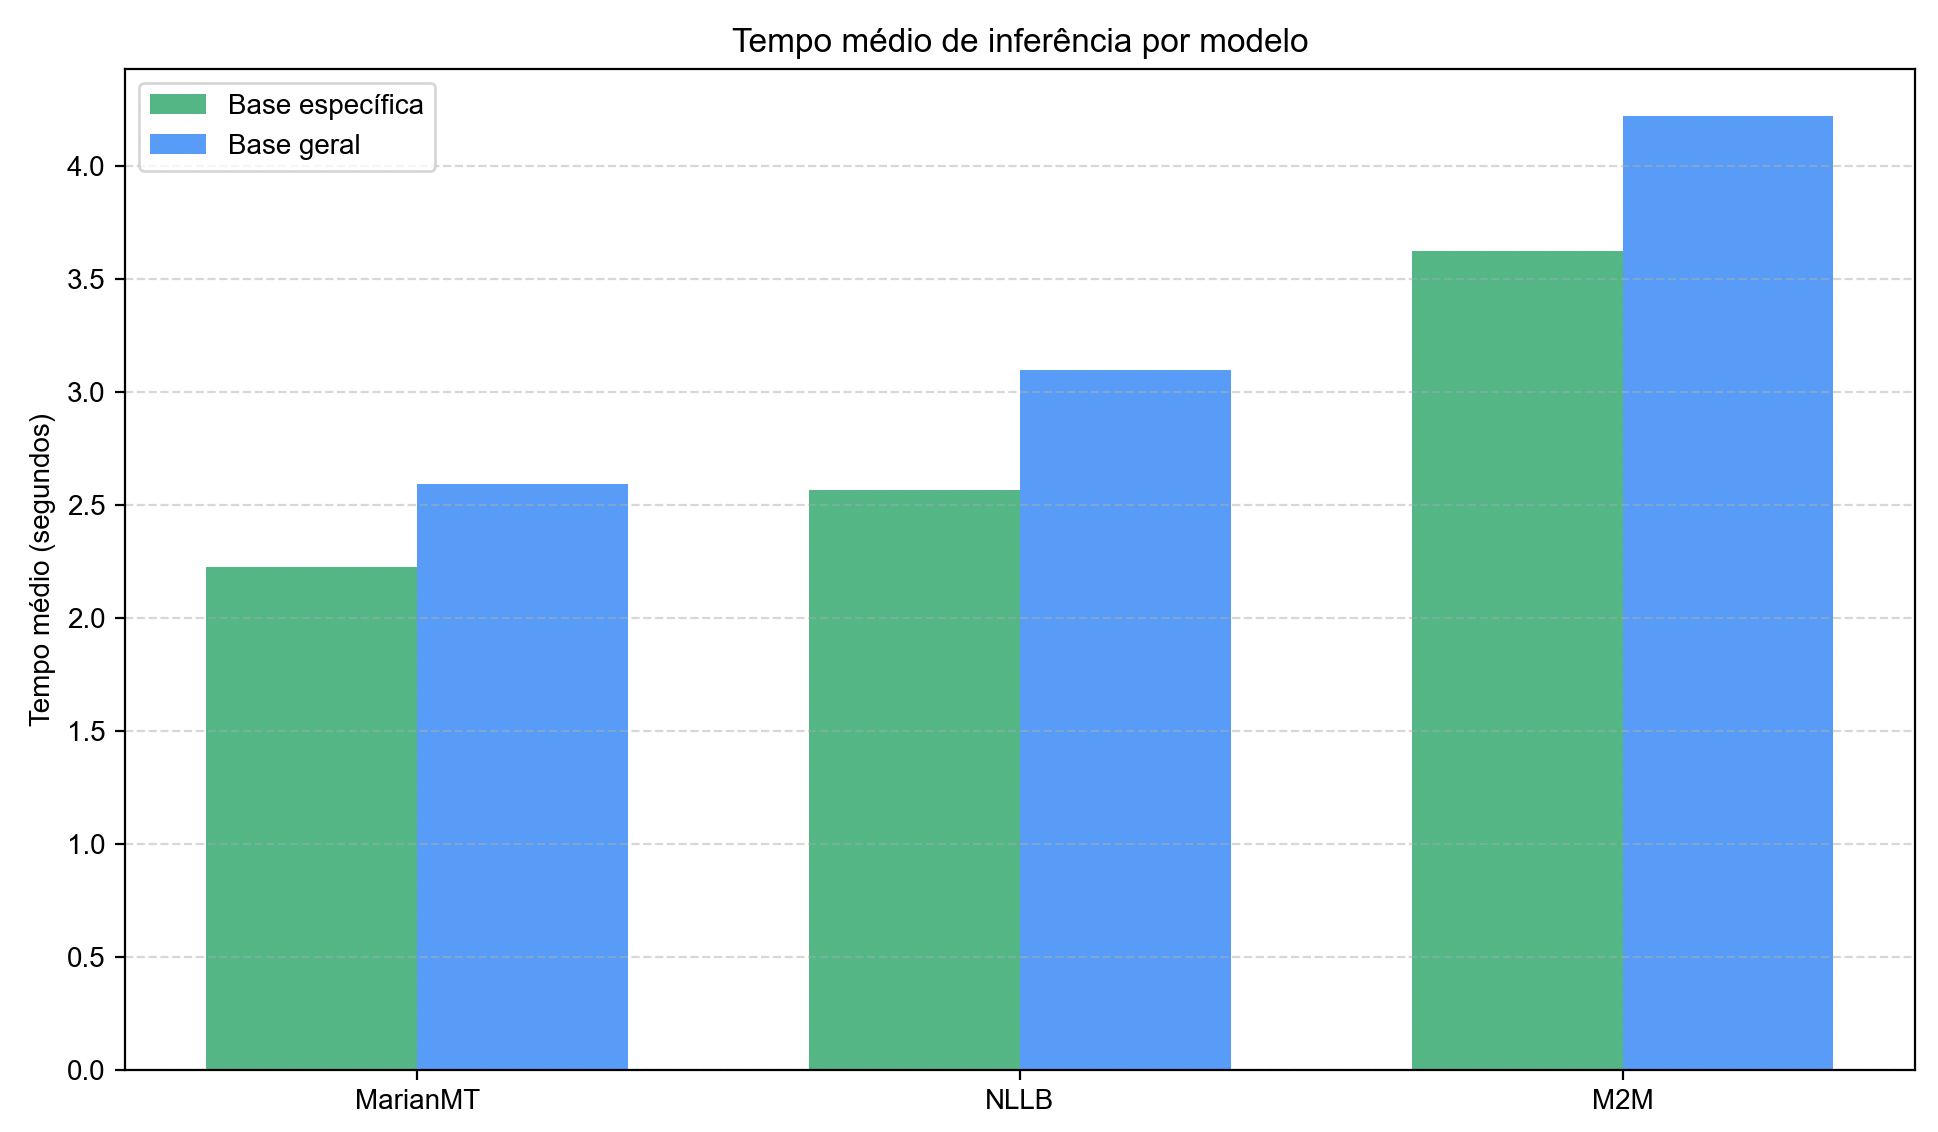
\includegraphics[width=0.9\textwidth]{Imagens/INFERENCE-TIME2.png}
    \caption{\label{fig:inference-time} Tempo de inferência por modelo e tipo de texto}
    \legend{Fonte: autor}
\end{figure}

Em relação ao uso médio de CPU, o MarianMT apresentou os menores valores nos dois tipos de texto, com 53,8\% para os textos gerais e 55,7\% para os textos específicos. O NLLB apresentou valores de 61,4\% e 62,2\%, respectivamente, enquanto o M2M100 apresentou os maiores valores, com 71,5\% nos textos gerais e 73,6\% nos textos específicos.

Observa-se, portanto, uma diferença considerável entre os modelos. O M2M100 apresentou uso médio de CPU superior ao MarianMT nos dois cenários, enquanto o NLLB permaneceu em uma posição intermediária.

Em relação ao pico de memória RAM, os resultados foram bastante próximos entre os modelos. Para textos gerais, os valores variaram de aproximadamente 6,24 GB a 6,25 GB, enquanto para textos específicos variaram de 6,26 GB a 6,27 GB. Ressalta-se que cada modelo foi executado separadamente, em um novo processo, sem execução simultânea ou reaproveitamento do processo utilizado pelos demais modelos. A proximidade dos valores ocorre porque a medição considera a memória residente total do processo durante a execução, incluindo o interpretador, as bibliotecas, os componentes auxiliares e as áreas temporárias de processamento, e não apenas a memória ocupada pelos parâmetros do modelo. Assim, o tamanho do modelo, isoladamente, não determina a variação observada no pico de memória nessa medição.

Quanto ao tempo de inferência, o MarianMT apresentou novamente o menor tempo nos dois tipos de texto. Para textos gerais, foram necessários 2,592 segundos, enquanto o NLLB apresentou 3,095 segundos e o M2M100 4,217 segundos. Para textos específicos, os tempos foram de 2,222 segundos para o MarianMT, 2,563 segundos para o NLLB e 3,621 segundos para o M2M100.

Os resultados indicam que, nas condições experimentais adotadas, o MarianMT apresentou o menor custo computacional entre os modelos avaliados considerando o uso médio de CPU e o tempo de inferência. O M2M100, por outro lado, apresentou os maiores valores dessas duas métricas.

Considerando conjuntamente os resultados de qualidade e eficiência computacional, observa-se que o MarianMT apresentou os maiores valores nas três métricas de qualidade avaliadas e, simultaneamente, os menores valores de uso médio de CPU e tempo de inferência. Esse comportamento o diferencia dos demais modelos nas condições estabelecidas neste experimento.

\section{Relação entre métricas}

As Tabelas \ref{table-metrics-general} e \ref{table-metrics-specific} apresentam as médias obtidas pelos modelos nas métricas BLEU, BERTScore e chrF para os textos gerais e específicos, respectivamente. A comparação conjunta dos resultados permite verificar se as métricas apresentam tendências semelhantes na avaliação dos modelos.

\begin{table}[htbp]
  \centering
  \caption{Relação entre a médias das métricas para textos gerais}
  \vspace{0.5em}
  \label{table-metrics-general}
  \setlength{\tabcolsep}{3pt}
  \begin{tabularx}{\textwidth}{>{\raggedright\arraybackslash}X l r r r r r}
    \toprule
    \textbf{Modelo} & \textbf{Base} & \textbf{BERTScore} & \textbf{BLEU} & \textbf{chrf} \\
    \midrule
    Helsinki-NLP/\penalty0opus-mt-tc-big-en-pt & Geral & 0,921 & 0,384 & 72,185 \\
    \addlinespace
    facebook/\penalty0nllb-200-distilled-600M & Geral & 0,903 & 0,303 &  66,196 \\
    \addlinespace
    facebook/\penalty0m2m100\_418M & Geral & 0,906 & 0,324 & 65,683 \\
    \bottomrule
  \end{tabularx}
\end{table}


\begin{table}[htbp]
  \centering
  \caption{Relação entre a médias das métricas para textos específicos}
  \vspace{0.5em}
  \label{table-metrics-specific}
  \setlength{\tabcolsep}{3pt}
  \begin{tabularx}{\textwidth}{>{\raggedright\arraybackslash}X l r r r r r}
    \toprule
    \textbf{Modelo} & \textbf{Base} & \textbf{BERTScore} & \textbf{BLEU} & \textbf{chrf} \\
    \midrule
    Helsinki-NLP/\penalty0opus-mt-tc-big-en-pt & Específico & 0,883 &  0,258 & 58,676 \\
    \addlinespace
    facebook/\penalty0nllb-200-distilled-600M & Específico & 0,875 & 0,217 &  55,235 \\
    \addlinespace
    facebook/\penalty0m2m100\_418M & Específico &  0,869 & 0,218 & 53,842 \\
    \bottomrule
  \end{tabularx}
\end{table}

Para os textos gerais, o MarianMT apresentou o maior valor nas três métricas consideradas, com BERTScore de 0,921, BLEU de 0,384 e chrF de 72,185. O NLLB e o M2M100 apresentaram valores inferiores, embora a posição relativa entre esses dois modelos varie de acordo com a métrica. Enquanto o M2M100 apresentou valor de BLEU superior ao NLLB, o NLLB apresentou valor de chrF superior ao M2M100. Os valores de BERTScore também foram próximos entre os dois modelos.Nos textos específicos, o MarianMT novamente apresentou os maiores valores nas três métricas. O modelo obteve BERTScore de 0,883, BLEU de 0,258 e chrF de 58,676. O NLLB apresentou valores de 0,875, 0,217 e 55,235, respectivamente, enquanto o M2M100 apresentou 0,869, 0,218 e 53,842.


De maneira geral, observa-se que as três métricas apontam o MarianMT como o modelo com melhor desempenho nas condições avaliadas. Entretanto, pequenas diferenças na ordenação dos modelos NLLB e M2M100 demonstram que os indicadores não produzem resultados completamente equivalentes. Esse comportamento está relacionado às características distintas de cada métrica, que avaliam diferentes aspectos da similaridade entre a tradução produzida e a referência.

Além da comparação entre os modelos, verifica-se que os valores das três métricas foram menores nos textos específicos em relação aos textos gerais. Esse comportamento foi observado para todos os modelos avaliados, reforçando a influência do tipo de texto sobre o desempenho dos modelos nas condições experimentais deste trabalho.